\documentclass[a4paper,11pt]{article}
\pdfoutput=1 % arXiv: force pdflatex
\usepackage{jheppub}
\usepackage[T1]{fontenc}
\usepackage{amsmath,amssymb,mathtools}
\usepackage{slashed}
\usepackage{graphicx}
\usepackage{booktabs}
\usepackage{cleveref} % "eq. (2.1)"; use \Cref at sentence start

% Project-wide notation. Define every symbol used more than once here, so
% notation changes are one-line edits. Keep in sync with notes/conventions.md.

\usepackage{xspace}

% --- general ---
\newcommand{\dd}{\mathrm{d}}
\newcommand{\order}[1]{\mathcal{O}\!\left(#1\right)}
\newcommand{\GeV}{\,\mathrm{GeV}}
\newcommand{\TeV}{\,\mathrm{TeV}}
\newcommand{\pb}{\,\mathrm{pb}}
\newcommand{\fb}{\,\mathrm{fb}}
\newcommand{\eg}{e.g.\@\xspace}
\newcommand{\ie}{i.e.\@\xspace}

% --- physics ---
\newcommand{\MSbar}{\overline{\mathrm{MS}}}
\newcommand{\aem}{\alpha}
\newcommand{\as}{\alpha_s}
\newcommand{\sqrts}{\sqrt{s}}
\newcommand{\Tr}{\operatorname{Tr}}

% --- editing (remove before submission; `grep -n '\\todo' sections/*.tex`) ---
\usepackage{xcolor}
\newcommand{\todo}[1]{{\color{red}[TODO: #1]}}
\newcommand{\authnote}[2]{{\color{blue}[#1: #2]}} % \authnote{initials}{comment}

% generated by `make values` -- do not edit

\newcommand{\valSqrtSRef}{\ensuremath{10\,\mathrm{GeV}}}  % 01_ee_mumu.json
\newcommand{\valSigmaTotMma}{\ensuremath{868.5\,\mathrm{pb}}}  % 01_ee_mumu.json
\newcommand{\valSigmaTotNum}{\ensuremath{868.5\,\mathrm{pb}}}  % 02_ee_mumu_numerics.json
\newcommand{\valSigmaRelDiff}{\ensuremath{2.2\times 10^{-16}}}  % 02_ee_mumu_numerics.json
\newcommand{\valAFB}{\ensuremath{0}}  % 02_ee_mumu_numerics.json
 % numbers from calc/ -- see results/*.json

\graphicspath{{figures/}}

\title{\boldmath Project title}

\author[a]{First Author,}
\author[b]{Second Author}

\affiliation[a]{Departamento de F\'isica, Universidad de Oviedo,\\
  C. Federico Garc\'ia Lorca 18, 33007 Oviedo, Spain}
\affiliation[b]{Institution,\\Address}

\emailAdd{first.author@uniovi.es}
\emailAdd{second.author@example.org}

\abstract{Abstract goes here.}

\begin{document}
\maketitle
\flushbottom

\section{Introduction}
\label{sec:introduction}

Motivation, state of the art, and what this paper does.
Example citation: the Standard Model~\cite{Weinberg:1967tq}.

The rest of the paper is organised as follows. In \cref{sec:setup} we\ldots

\section{Setup}
\label{sec:setup}

% EXAMPLE content -- shows how analytic results flow from Mathematica into the paper.
% Equations below are \input from paper/generated/, written by
% calc/mathematica/scripts/01_ee_mumu.wl. Never edit generated files by hand.

As a worked example we consider $e^+e^-\to\mu^+\mu^-$ at tree level in massless
QED. Summing over spins with explicit Dirac traces gives
\begin{equation}
  \frac{\dd\sigma}{\dd\Omega} = % generated by calc/mathematica -- do not edit
\frac{\alpha ^2 \left(\cos ^2(\theta )+1\right)}{4 s}
\,,
  \label{eq:dsigma}
\end{equation}
which integrates to
\begin{equation}
  \sigma = % generated by calc/mathematica -- do not edit
\frac{4 \pi  \alpha ^2}{3 s}
\,.
  \label{eq:sigmatot}
\end{equation}

\section{Results}
\label{sec:results}

% EXAMPLE content -- numbers are \val... macros from paper/generated/values.tex.

At $\sqrts = \valSqrtSRef$ the total cross section from \cref{eq:sigmatot} is
$\sigma = \valSigmaTotMma$. Integrating \cref{eq:dsigma} numerically in Python
gives $\valSigmaTotNum$, a relative difference of $\valSigmaRelDiff$, and a
forward--backward asymmetry $A_\text{FB} = \valAFB$ as expected for pure QED.
The angular distribution is shown in \cref{fig:dsigma}.

\begin{figure}[t]
  \centering
  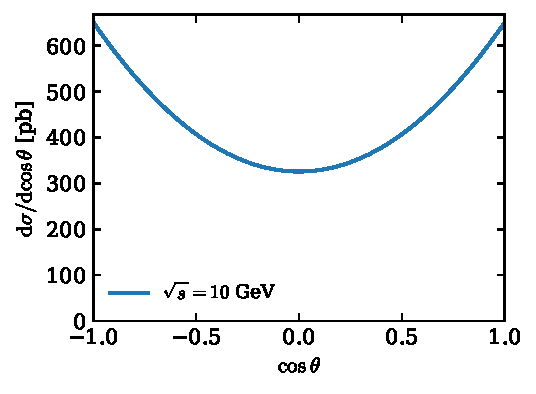
\includegraphics{ee_mumu_dsigma}
  \caption{Angular distribution of $e^+e^-\to\mu^+\mu^-$ at $\sqrts=\valSqrtSRef$.}
  \label{fig:dsigma}
\end{figure}

\section{Conclusions}
\label{sec:conclusions}

Summary and outlook.


\acknowledgments
Acknowledgments and funding.

\appendix
\section{Conventions}
\label{app:conventions}

We use natural units $\hbar=c=1$ and the metric $g_{\mu\nu}=\mathrm{diag}(+1,-1,-1,-1)$.


\bibliographystyle{JHEP}
\bibliography{references}

\end{document}
